% Textbook Section 2.4, pp. 150--156.
\section[Partitioned matrices]{Partitioned Matrices}

% \sectioncard{2.4}{Partitioned Matrices\\[-.25ex]{\}}

\begin{frame}{Why Partition a Matrix?}
    Suppose we have three modules in a circuit with tons of connections:
    \begin{figure}
        \centering
        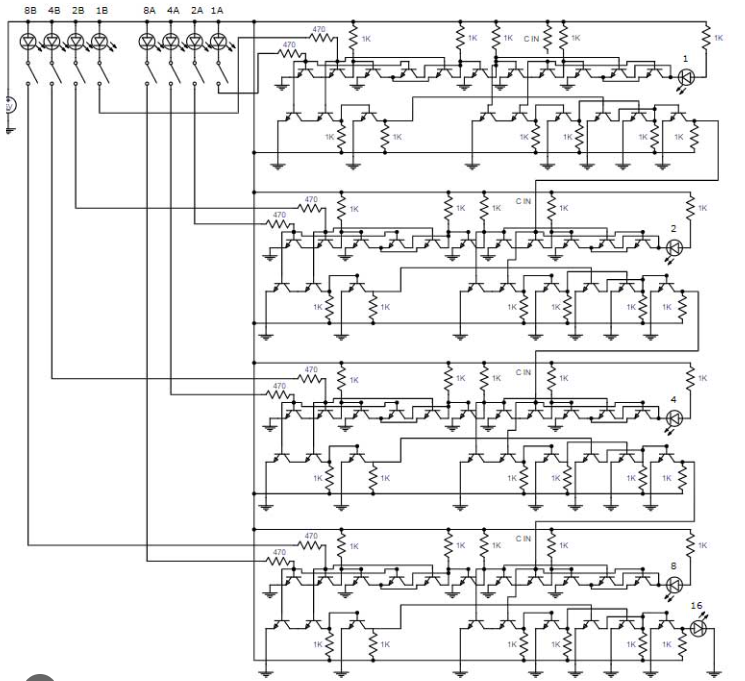
\includegraphics[height=.8\textheight]{example.png}
    \end{figure}

\end{frame}

\begin{frame}{Why Partition a Matrix?}
    Suppose we have three modules (chips) that does :+, -, *. Their connection can be described with:
\[
A=\begin{bmatrix}
A_{11}&A_{12}&A_{13}\\
A_{21}&A_{22}&A_{23}\\
A_{31}&A_{32}&A_{33}
\end{bmatrix}.
\]
\pause
The diagonal blocks describe the three chips. The off-diagonal blocks describe their interconnections.
\medskip
\begin{block}{Computational motivation}
Block algorithms let a computer work with a few submatrices at a time. High-performance numerical software uses partitioned calculations extensively.
\end{block}
\end{frame}

\begin{frame}{Reading the Blocks}
\[
A=\left[
\begin{array}{ccc:cc:c}
3&0&1&5&9&2\\
5&2&4&0&3&1\\ \hdashline
8&6&3&1&7&4
\end{array}\right]
=\begin{bmatrix}
A_{11}&A_{12}&A_{13}\\
A_{21}&A_{22}&A_{23}
\end{bmatrix}.
\]
\pause
\[
A_{11}=\begin{bmatrix}3&0&1\\5&2&4\end{bmatrix},\quad
A_{12}=\begin{bmatrix}5&9\\0&3\end{bmatrix},\quad
A_{13}=\begin{bmatrix}2\\1\end{bmatrix},
\]
\[
A_{21}=\begin{bmatrix}8&6&3\end{bmatrix},\quad
A_{22}=\begin{bmatrix}1&7\end{bmatrix},\quad
A_{23}=\begin{bmatrix}4\end{bmatrix}.
\]
\pause
Horizontal, vertical, and rectangular partitions may all describe the same matrix. Each block is itself a matrix, so its dimensions \textbf{matter}.
\end{frame}

\begin{frame}{Addition and Scalar Multiplication}
If $A$ and $B$ have the same size and exactly the same partition, then
\[
\begin{bmatrix}A_{11}&A_{12}\\A_{21}&A_{22}\end{bmatrix}
+
\begin{bmatrix}B_{11}&B_{12}\\B_{21}&B_{22}\end{bmatrix}
=
\begin{bmatrix}
A_{11}+B_{11}&A_{12}+B_{12}\\
A_{21}+B_{21}&A_{22}+B_{22}
\end{bmatrix}.
\]
\pause
Scalar multiplication also acts block by block:
\[
c\begin{bmatrix}A_{11}&A_{12}\\A_{21}&A_{22}\end{bmatrix}
=\begin{bmatrix}cA_{11}&cA_{12}\\cA_{21}&cA_{22}\end{bmatrix}.
\]
\end{frame}

\begin{frame}[shrink=3]{Conformable Partitions}
\[
A=\left[\begin{array}{ccc|cc}
2&-3&1&0&-4\\
1&5&-2&3&-1\\ \hline
0&-4&-2&7&-1
\end{array}\right]
=\begin{bmatrix}A_{11}&A_{12}\\A_{21}&A_{22}\end{bmatrix},
\]
\[
B=\left[\begin{array}{cc}6&4\\-2&1\\-3&7\\ \hline -1&3\\5&2\end{array}\right]
=\begin{bmatrix}B_1\\B_2\end{bmatrix}.
\]
The column partition of $A$ matches the row partition of $B$, so the partitions are conformable.
\pause
\[
AB=
\begin{bmatrix}A_{11}&A_{12}\\A_{21}&A_{22}\end{bmatrix}
\begin{bmatrix}B_1\\B_2\end{bmatrix}
=\begin{bmatrix}
A_{11}B_1+A_{12}B_2\\
A_{21}B_1+A_{22}B_2
\end{bmatrix}.
\]
\end{frame}

\begin{frame}{The Upper Block}
\small
\[
A_{11}B_1=
\begin{bmatrix}2&-3&1\\1&5&-2\end{bmatrix}
\begin{bmatrix}6&4\\-2&1\\-3&7\end{bmatrix}
=\begin{bmatrix}15&12\\2&-5\end{bmatrix},
\]
\pause
\[
A_{12}B_2=
\begin{bmatrix}0&-4\\3&-1\end{bmatrix}
\begin{bmatrix}-1&3\\5&2\end{bmatrix}
=\begin{bmatrix}-20&-8\\-8&7\end{bmatrix}.
\]
\pause
\[
A_{11}B_1+A_{12}B_2=\begin{bmatrix}-5&4\\-6&2\end{bmatrix}.
\]
\end{frame}

\begin{frame}{Completing the Block Product}
The lower block is
\[
A_{21}B_1+A_{22}B_2=
\begin{bmatrix}0&-4&-2\end{bmatrix}\begin{bmatrix}6&4\\-2&1\\-3&7\end{bmatrix}+\begin{bmatrix}7&-1\end{bmatrix}\begin{bmatrix}-1&3\\5&2\end{bmatrix}=
\]
\[
=\begin{bmatrix}14&-18\end{bmatrix}+\begin{bmatrix}-12&19\end{bmatrix}=
\begin{bmatrix}2&1\end{bmatrix}.
\]
\pause
Therefore
\[
AB=
\begin{bmatrix}A_{11}&A_{12}\\A_{21}&A_{22}\end{bmatrix}
\begin{bmatrix}B_1\\B_2\end{bmatrix}
=\begin{bmatrix}
A_{11}B_1+A_{12}B_2\\
A_{21}B_1+A_{22}B_2
\end{bmatrix}
=\begin{bmatrix}-5&4\\-6&2\\2&1\end{bmatrix}.
\]
The block rule is the usual row-column rule with matrices in place of scalars. Factor order remains fixed.
\end{frame}

\begin{frame}[shrink=8]{A Sum of Outer Products}
Let
\[
A=\begin{bmatrix}-3&1&2\\1&-4&5\end{bmatrix},\qquad
B=\begin{bmatrix}a&b\\c&d\\e&f\end{bmatrix}.
\]
\pause
Partition $A$ by columns and $B$ by rows:
\[
AB=\operatorname{col}_1(A)\operatorname{row}_1(B)
+\operatorname{col}_2(A)\operatorname{row}_2(B)
+\operatorname{col}_3(A)\operatorname{row}_3(B).
\]
\pause
\[
=\begin{bmatrix}-3a&-3b\\a&b\end{bmatrix}
+\begin{bmatrix}c&d\\-4c&-4d\end{bmatrix}
+\begin{bmatrix}2e&2f\\5e&5f\end{bmatrix}
\]
\[
=\begin{bmatrix}-3a+c+2e&-3b+d+2f\\a-4c+5e&b-4d+5f\end{bmatrix}.
\]
\end{frame}

\begin{frame}[shrink=5]{Theorem 10: Column-Row Expansion}
If $A$ is $m\times n$ and $B$ is $n\times p$, then
\[
AB=\sum_{k=1}^{n}\operatorname{col}_k(A)\operatorname{row}_k(B).
\]
The $(i,j)$ entry in this sum is
\[
a_{i1}b_{1j}+a_{i2}b_{2j}+\cdots+a_{in}b_{nj},
\]
which is exactly the $(i,j)$ entry given by the row-column rule.
% \pause
% \begin{block}{Textbook Practice Problem 2}
% If $X=[\,X_1\ X_2\,]$, then
% \[
% X^TX=
% \begin{bmatrix}
% X_1^TX_1&X_1^TX_2\\
% X_2^TX_1&X_2^TX_2
% \end{bmatrix}.
% \]
% \end{block}
\end{frame}

\begin{frame}[shrink=4]{The Block Equations}
Let
\[
A=\begin{bmatrix}A_{11}&A_{12}\\0&A_{22}\end{bmatrix},\qquad
A^{-1}=B=\begin{bmatrix}B_{11}&B_{12}\\B_{21}&B_{22}\end{bmatrix}.
\]
From $AB=I$,
\[
\begin{aligned}
A_{11}B_{11}+A_{12}B_{21}&=I, &
A_{11}B_{12}+A_{12}B_{22}&=0,\\
A_{22}B_{21}&=0, &
A_{22}B_{22}&=I.
\end{aligned}
\]
\pause
The Invertible Matrix Theorem gives
\[
B_{22}=A_{22}^{-1},\quad B_{21}=0,\quad B_{11}=A_{11}^{-1},\quad
B_{12}=-A_{11}^{-1}A_{12}A_{22}^{-1}.
\]
\end{frame}

\begin{frame}{The Inverse Formula}
Thus
\[
\boxed{
A^{-1}=\begin{bmatrix}
A_{11}^{-1}&-A_{11}^{-1}A_{12}A_{22}^{-1}\\
0&A_{22}^{-1}
\end{bmatrix}}.
\]
\pause
A block diagonal matrix is invertible exactly when each diagonal block is invertible. In particular,
\[
\begin{bmatrix}I&0\\A&I\end{bmatrix}^{-1}
\] is\pause
\[
=\begin{bmatrix}I&0\\-A&I\end{bmatrix}.
\]
\end{frame}
